\documentclass[12pt,a4paper]{article}
\usepackage[utf8]{inputenc}
\usepackage{amsmath}
\usepackage{amsfonts}
\usepackage{amssymb}
\usepackage{listings}
\usepackage{url}
\usepackage[bulgarian]{babel}
\usepackage{listings}
\usepackage{enumerate}
\usepackage{hyperref}
\usepackage[framemethod=tikz]{mdframed}
\usepackage{relsize}


\newcommand{\code}[1]{\texttt{#1}}

\lstset{breaklines=true}


\author{\textit{email: kalin@fmi.uni-sofia.bg}}
\title{\textsc{Задачи за задължителна самоподготовка} \\
по \\
Обектно-ориентирано програмиране\\
\textit{Функции от високо ниво}}



\begin{document}
\maketitle


\begin{enumerate}


	\item Да се дефинира функция \code{double root ([подходящ тип]f, double a, double b, double e)}, където
	 $f:double \rightarrow double$ е непрекърсната и монотонна в интервала $[a,b]$ и притежава корен в него, а $e$ е положително число. Чрез използване на двоично търсене (\textit{bisection}), функцията \code{root} да намира приближение на корена на $f$ в интервала $[a,b]$ с грешка най-много $e$.

	\begin{mdframed}[hidealllines=true,backgroundcolor=gray!20]
	\relscale{0.75}
	Упътване:\\

	Установете дали функцията е растяща или намаляваща. Да приемем, че функцията е растяща. За намаляващи функции алгоритъмът е аналогичен. \\

	За всеки интервал $[a,b]$ имаме точно три възможни случая:\\

	\begin{center}
	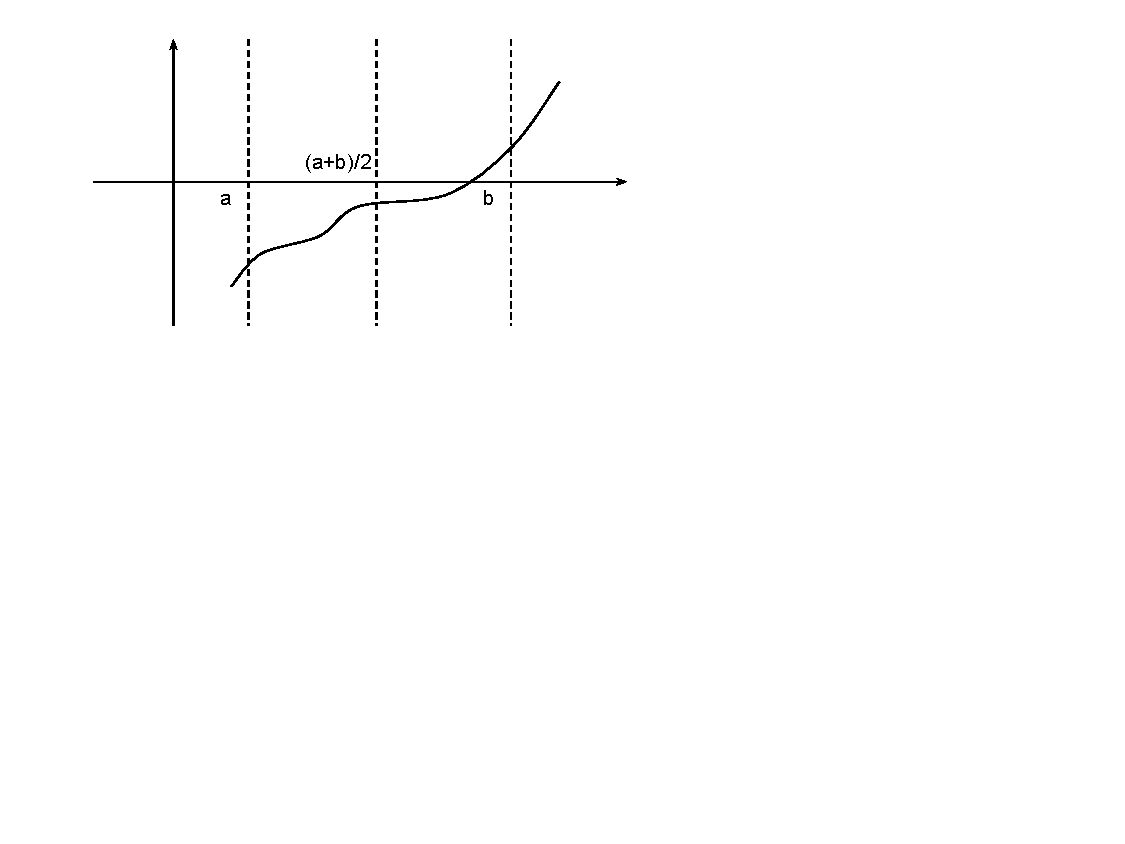
\includegraphics[width=14.0cm]{images/function}
	\end{center}

	\vspace{-180px}


	\begin{enumerate}
		\item $|f(\frac{a+b}{2})| < e$. В този случай приближението е намерено и то е $\frac{a+b}{2}$
		\item $f(\frac{a+b}{2}) < 0$. В този случай търсим корена на функцията в интервала $[\frac{a+b}{2},b]$
		\item $f(\frac{a+b}{2}) > 0$. В този случай търсим корена на функцията в интервала $[a,\frac{a+b}{2}]$
	\end{enumerate}


	\end{mdframed}

	\begin{itemize}
		\item Дефинирайте два варианта на функцията: итеративен и рекурсивен.
		\item Тествайте функцията \code{root} с поне два примера.
	\end{itemize}


	\item Да се дефинира функция \code{void zip (double a1[], double a2[], double res[], int n, [подходящ тип]f)}, където \code{a1}, \code{a2} и \code{res} са масиви с \code{n} на брой елементи, а \code{f} е функция от тип $f:double \times double \rightarrow double$. Като резултат от работата на функцията елементите на \code{res} да съдържат стойностите на функцията \code{f} върху съответните елементи на \code{a1} и \code{a2}, така че $res[i]=f(a1[i],a2[i])$ за $i=0..n-1$.
	\begin{itemize}
		\item Тествайте функцията с поне два примера.
	\end{itemize}
	\item Функцията \code{zip} от предишната задача да се преобразува до шаблон, така че масивите \code{a1}, \code{a2} и \code{res} да са от произволен тип \code{T}.
	\begin{itemize}
		\item Тествайте функцията с поне два примера.
	\end{itemize}
	\item Функцията \code{zip} от предишната задача да се преобразува до шаблон, така че всеки от масивите \code{a1}, \code{a2} и \code{res} да са от различни помежду си типове $T_1$, $T_2$ и $T_3$, а $f:T_1 \times T_2 \rightarrow T_3$.
	\begin{itemize}
		\item Тествайте функцията с поне два примера.
	\end{itemize}

\end{enumerate}







	\vspace{20px}


\end{document}
